\chapter{Vergelijking tussen algoritmes}
Hieronder volgen enkele vergelijkende tests tussen de vijf ge\"implementeerde algoritmes. Er zullen 2 soorten tests uitgevoerd worden. Als eerste wordt de compressieratio getest op verschillende teksten en worden deze resultaten ge\"interpreteerd. In een tweede test wordt de snelheid van de vijf algoritmes met elkaar vergeleken, voor zowel tekstuele als \texttt{random} data\footnote{Alle 256 extended ASCII tekens komen er in voor, waardoor elk karakter een code van 8 bits heeft.}. Tenslotte wordt er een afweging gemaakt van compressieratio en tijd om te bepalen in welke situaties welk algoritme gebruikt moet worden.

\section{Compressieratio}
De compressieratio wordt telkens gegeven door volgende formule:
$$ratio = \frac{c}{o}$$
Hierin staan $c$ en $o$ respectievelijk voor de grootte van het gecomprimeerde bestand en de originele bestandsgrootte. De tests voor compressieratio zullen enkel worden uitgevoerd op tekstuele data, aangezien random data zeer slecht tot zelfs niet gecomprimeerd kan worden. \cite{ad3cursus}.

\subsection{Testbestanden}
De bestanden die zullen getest worden, zijn de volgende:
\begin{itemize}
	\item \textbf{az: } Dit is een bestand dat sequentieel alle 26 letters van het alfabet bevat. Elke letter komt voor in groepen van $100\ 000$.
	\item \textbf{az\_s:} Dit is hetzelfde bestand als test \emph{az}, maar dan grondig door elkaar geschud. Op deze manier kan worden getest hoe het algoritme presteert op niet-sequenti\"ele tekst.
	\item \textbf{bible:} De \emph{King James} versie van de Bijbel. \cite{gutenbergbible} Aan de hand van deze test kan worden gemeten hoe goed het algoritme presteert op een willekeurige ``reguliere'' tekst.
	\item \textbf{kitten:} Een vergroting van figuur \ref{fig:cutekitten} naar $3\ 000$ pixels breedte en hoogte. De onderkant van deze afbeelding bevat enkel dezelfde tint rood(\texttt{\#ff0000}). De verwachting hiervoor is dat het \huffslid en \huffblock hier goed op zullen presteren. Het is belangrijk dat dit een \emph{bitmap}-afbeelding is, andere formaten zoals bijvoorbeeld \emph{JPEG}, hebben standaard al een compressie ingebouwd, waardoor de compressiealgoritmes hier niet goed op zullen presteren.
\end{itemize}

\begin{figure}[h]
	\centering
	
\includegraphics[width=0.3\linewidth]{resources/ratio-kitten.png}
	\label{fig:cutekitten}
	\caption{Deze afbeelding wordt gebruikt in de
	\emph{kitten}-test. \cite{cutekitten}}
\end{figure}
\newpage
\subsection{Interpretatie}
Na het uitvoeren van de tests werden volgende resultaten berekend. Uitzonderlijke waarden zijn in het \textbf{vet} aangeduid.
\begin{table}[h]
	\centering
	\begin{tabular}{|l||c|c|c|c|}
		\hline
		& \textbf{ad} & \textbf{ad\_s} & \textbf{bible} & \textbf{kitten}\\\hline
		\textbf{Standaard} & 59.62 \% & 59.62 \% & 57.91 \% & 76.76 \%\\
		\textbf{Adaptive} & 60.10 \% & 60.11 \% & 57.91 \% & 76.78 \%\\		
		\textbf{Sliding window} & \textbf{13.40 \%} & 60.10 \% & 57.82 \% & \textbf{69.87 \%}\\
		\textbf{Two-pass Adaptive} & 60.10 \% & 60.08 \% & 57.92 \% & 76.78 \%\\
		\textbf{Blockwise Adaptive} & \textbf{42.30 \%} & 60.11 \% & 57.88 \% & \textbf{71.85 \%}\\
		\hline
	\end{tabular}
	\label{tbl:compressieratios}
	\caption{Compressieratio's van de vijf algoritmes.}
\end{table}
\\Afgaande op de resultaten uit tabel \ref{tbl:compressieratios} merken we op dat voor gewone tekst, test \emph{bible}, alle algoritmes gelijkaardige compressieratio's behalen. \huffslid en \huffblock presteren zeer goed op de \emph{ad}-test zoals de bedoeling was. Voor de \emph{kitten}-test geldt hetzelfde, maar hier is dit minder duidelijk. Dit komt doordat het bestand naast de onderste rode sectie, wel nog veel verschillende kleuren bevat. Daardoor zal enkel het laatste stuk van de foto zeer goed gecomprimeerd kunnen worden, wat niet zo zwaar doorweegt in de uiteindelijke compressieratio. Tenslotte concluderen we uit de \emph{ad\_s}-test dat gerandomiseerde tekst zonder enige vorm van herhaling zeer slecht presteert bij alle algoritmes. Belangrijk om op te merken is dat het verschil met de \emph{bible}-test niet heel groot is.

\section{Snelheid}
Tenslotte wordt de snelheid van de verschillende algoritmes met elkaar vergeleken. Dit doen we zowel voor tekstuele data als voor random data, want het \huffstd werd geoptimaliseerd voor random data zoals reeds eerder vermeld. Bovendien vermoeden we dat de andere vier algoritmes die op het \huffadap gebaseerd zijn, hier veel slechter op zullen presteren omdat de codes langer zullen zijn. Voor elk meetresultaat wordt een bestand van de gegeven tekstgrootte eerst ge\"encodeerd en vervolgens gedecodeerd. Deze tests werden uitgevoerd op een \emph{Intel Core i3-4005U CPU met 4 cores, aan \SI{1.70}{\giga\hertz}}.
\begin{figure}[p]
	\centering
	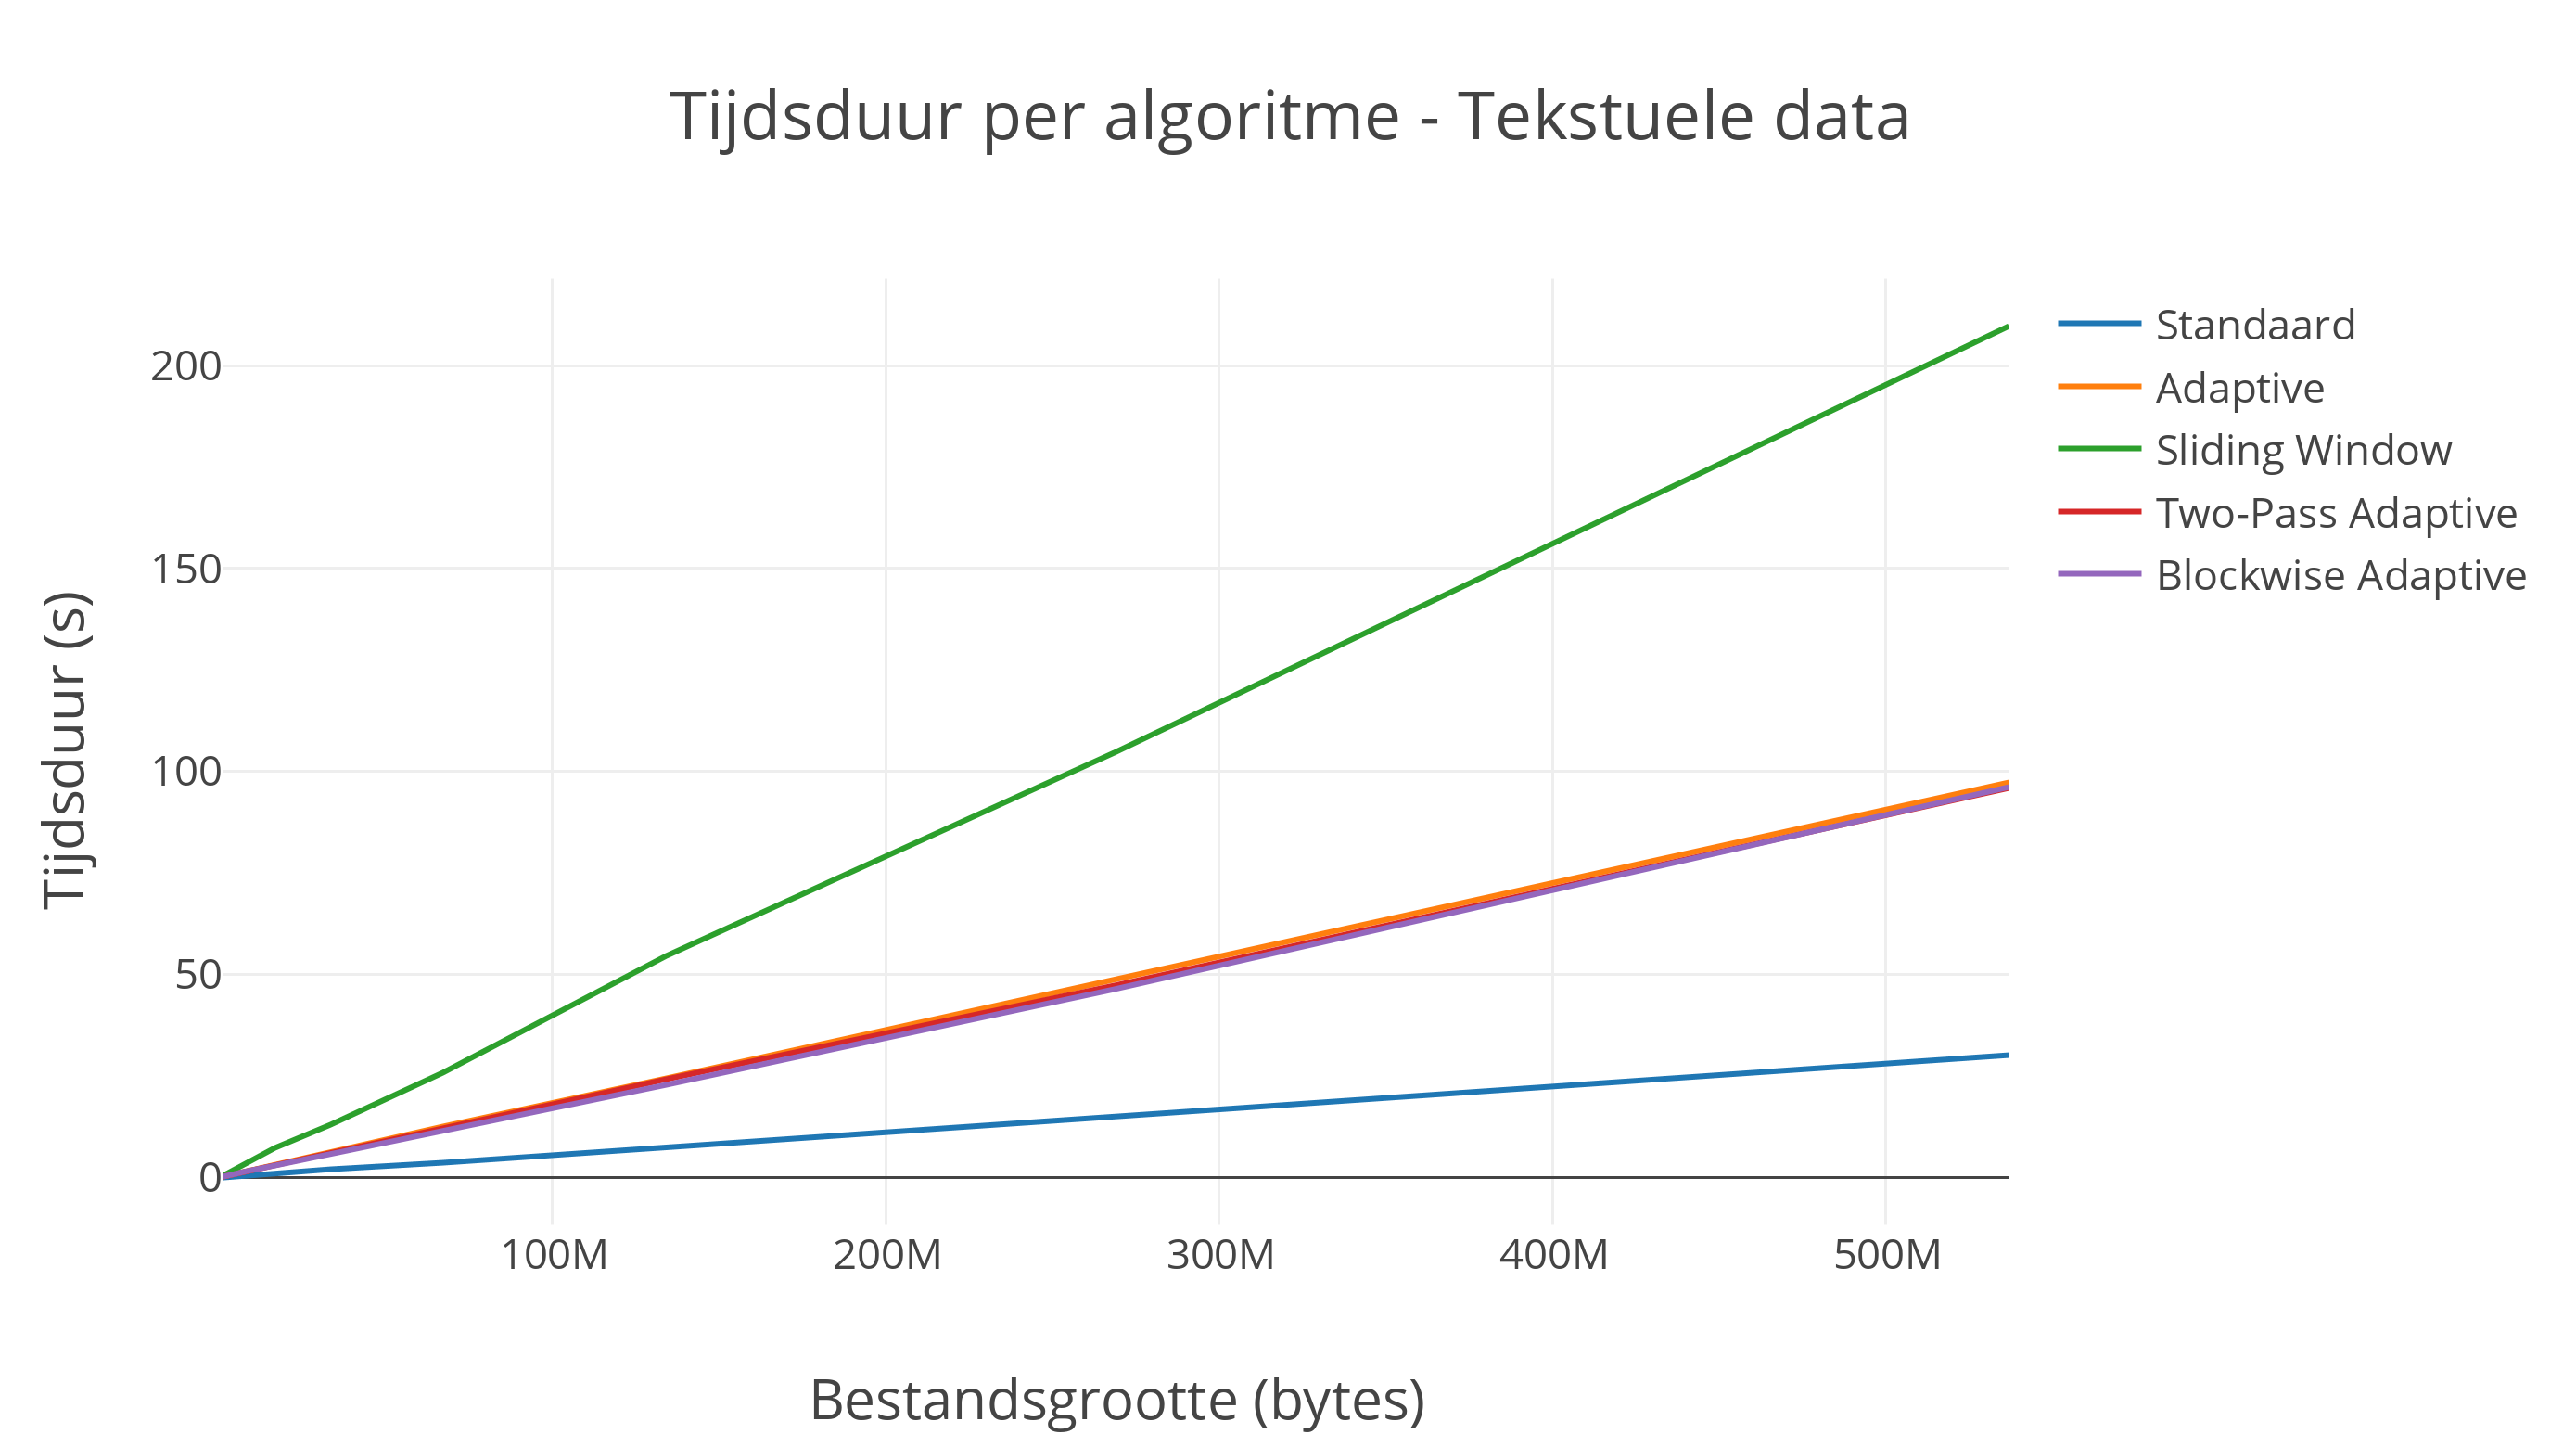
\includegraphics[width=\linewidth]{resources/timing-regular.png}
	\caption{Tijdsmeting voor tekstuele data}
\bigbreak
	\centering
	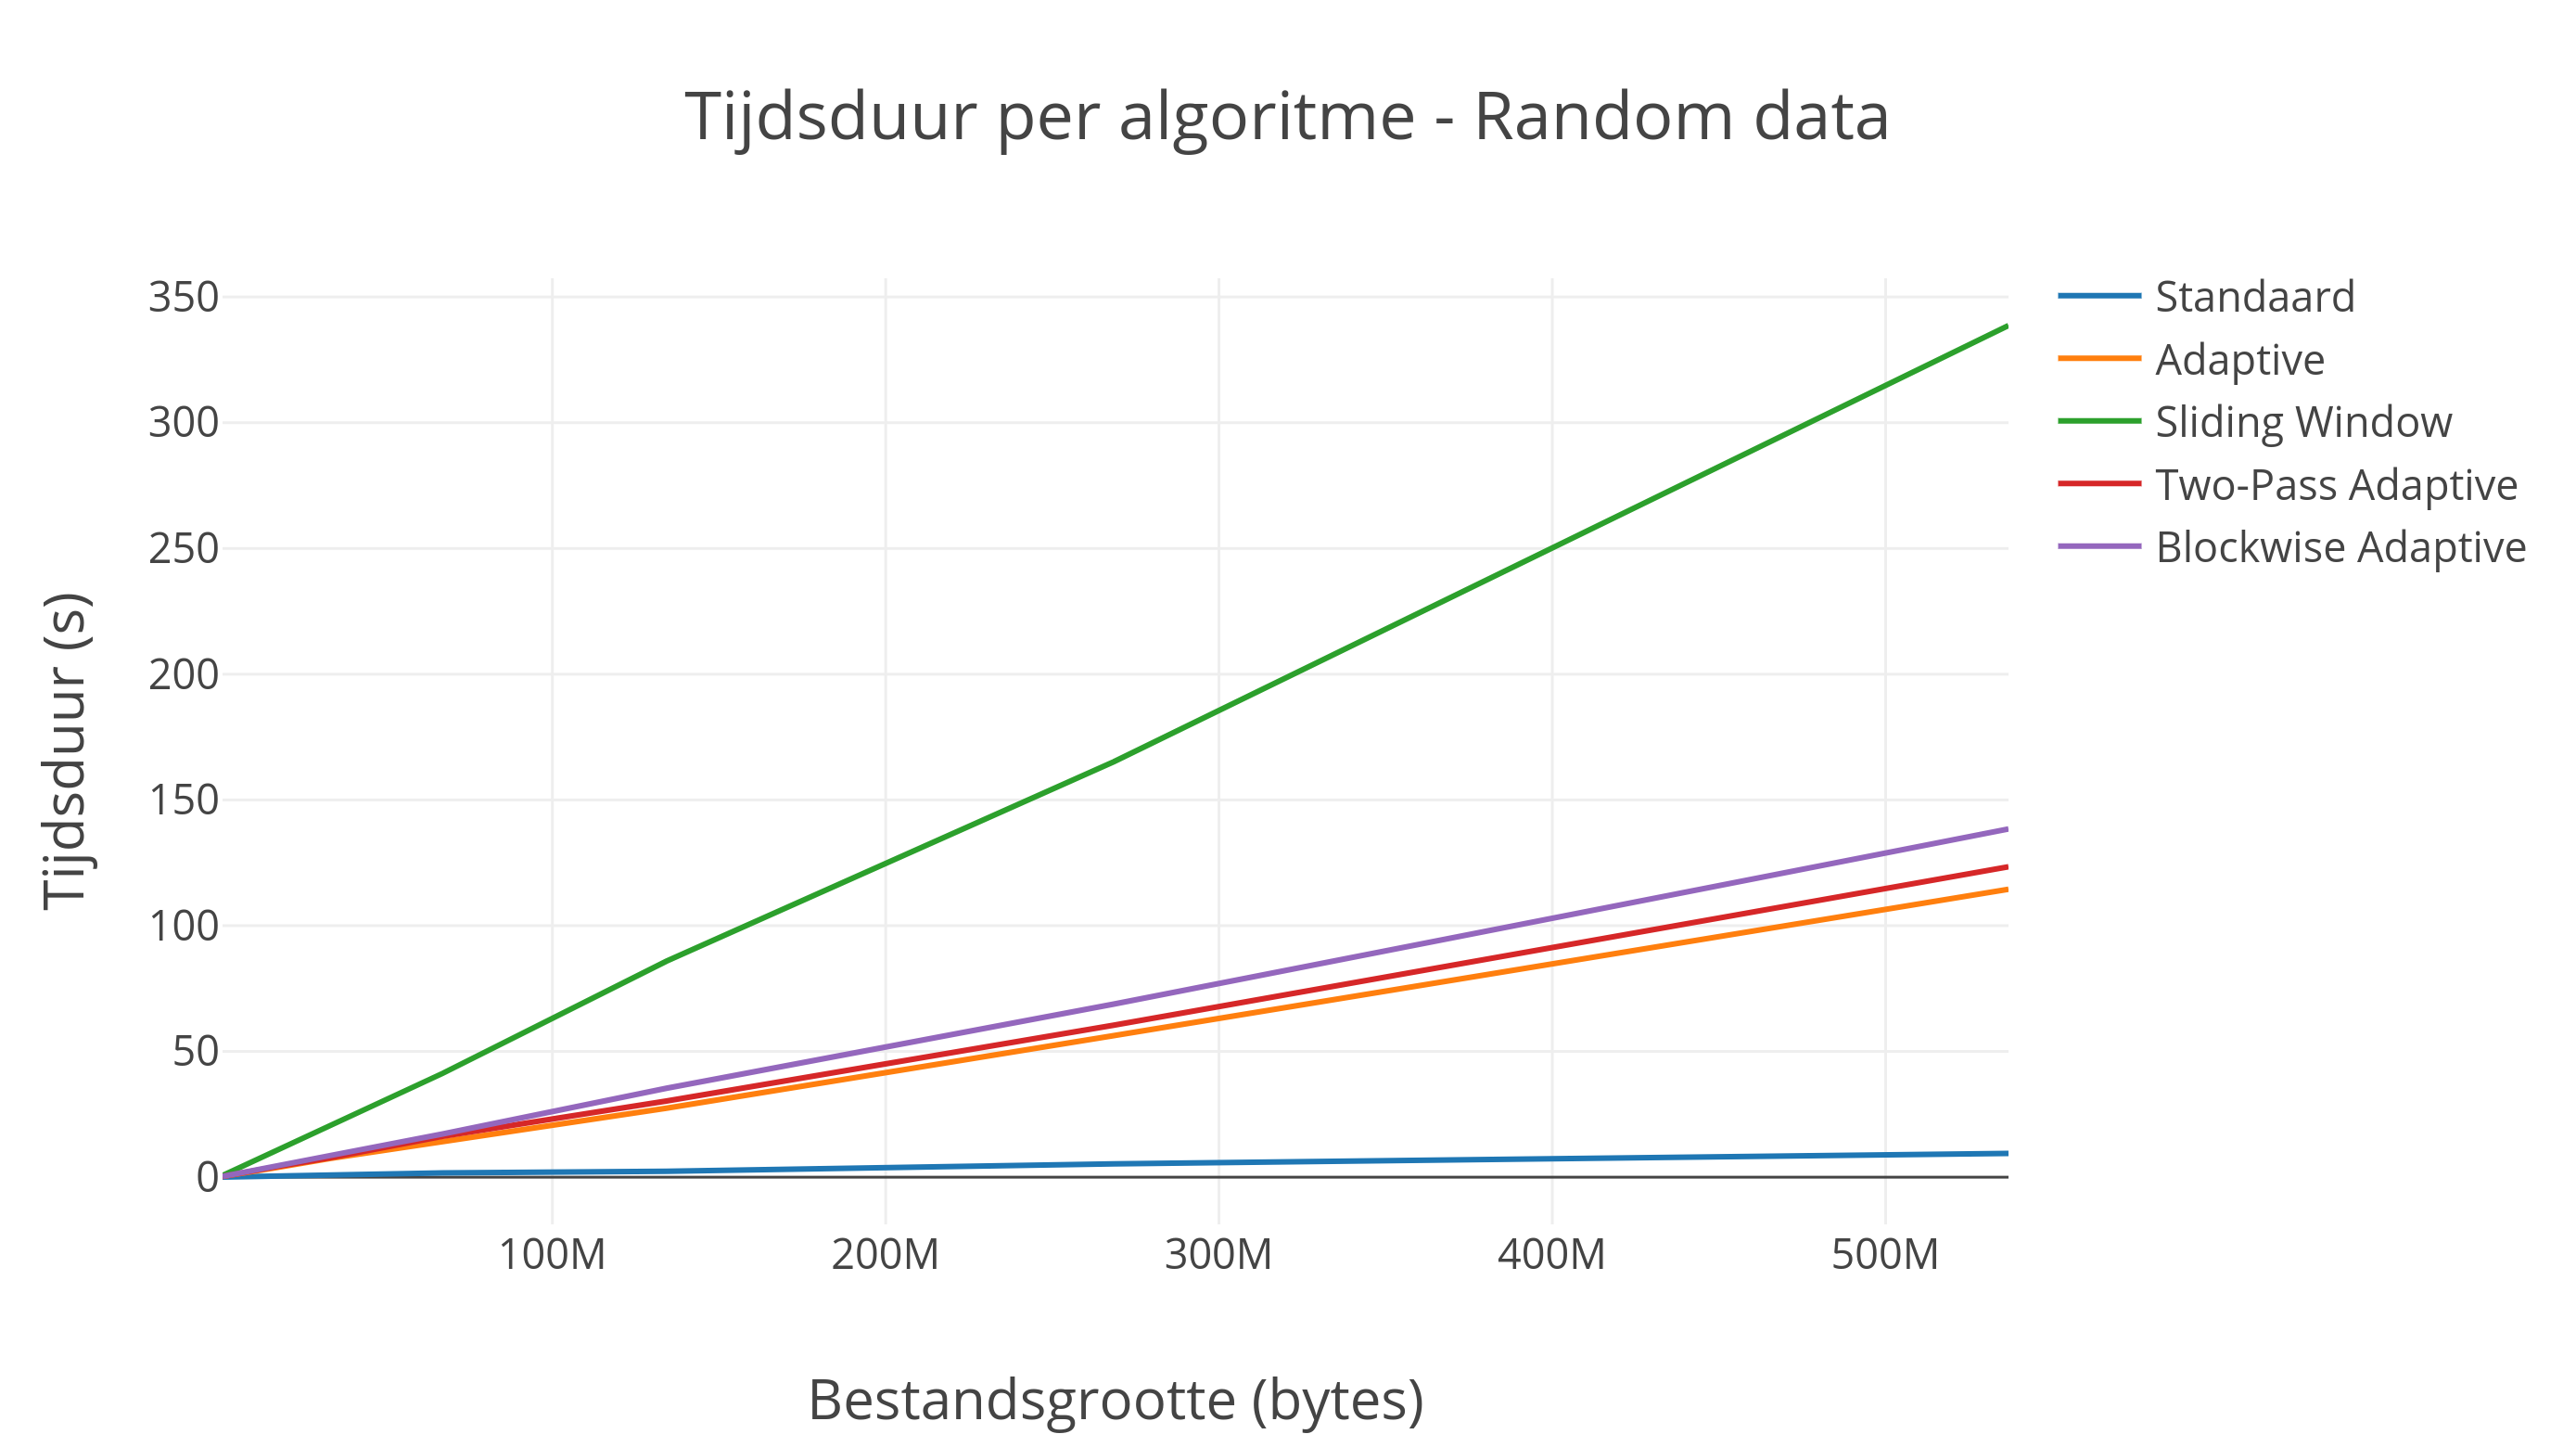
\includegraphics[width=\linewidth]{resources/timing-random.png}
	\caption{Tijdsmeting voor random data}
\end{figure}
\newpage
\noindent Het is onmiddellijk duidelijk dat de uitvoeringstijd lineair stijgt naarmate de lengte van de invoer groter wordt, zoals verwacht. Het vermoeden dat alle algoritmes, behalve het \huffstd veel slechter presteren op random data dan op tekstuele data wordt bevestigd. Bovendien merken we op dat het \huffslid bijzonder slecht presteert, meer dan dubbel zo slecht dan de andere drie \emph{Adaptive}-algoritmes. Voor random data valt dit eenvoudig te verklaren: Alle 256 ASCII karakters komen er in voor, dus de boom zal zeer groot zijn. Aangezien alle karakters ook even vaak voorkomen en het \emph{sliding window} een grootte heeft van $15 000$, zal het nooit voorkomen dat een karakter volledig uit de boom verwijderd wordt. Door deze grote boom zullen de swap operaties zeer duur zijn, wat de grootste kost van het algoritme is.

\section{Use-cases per algoritme}
\begin{enumerate}
	\item \textbf{Standaard:} Het grote voordeel van dit algoritme is dat het zeer snel werkt en goed presteert op reguliere data. Een belangrijk nadeel is echter wel dat het niet offline kan worden gebruikt en dus beperkt is in de hoeveelheid die in één keer gecomprimeerd kan worden.
	\item \textbf{Adaptive:} Zeer goed wanneer \huffstd niet kan worden gebruikt, bijvoorbeeld omdat de data online moet worden gecomprimeerd.
	\item \textbf{Sliding window:} Dit algoritme presteert zeer goed indien er veel spatiale lokaliteit is. Er moet echter wel rekening mee worden gehouden dat de snelheid zeer laag ligt.
	\item \textbf{Two-pass adaptive:} De compressieratio is in het algemeen het slechtst, doordat de boom en de gewichten moeten worden doorgestuurd. De snelheid is vergelijkbaar met \huffadap, er zijn dus geen voordelen aan dit algoritme.
	\item \textbf{Blockwise adaptive:} Presteert iets minder goed als \huffslid, maar is wel veel sneller. Bij voorkeur wordt dus dit algoritme gebruikt in plaats van \huffslid, op voorwaarde dat een verlies aan compressieratio toegelaten is.
\end{enumerate}